% szablon sprawozdania z dnia 2020-10-27
\documentclass{article} % mwart , article
\usepackage[polish]{babel}
\usepackage[utf8]{inputenc}	
\usepackage{polski}	
\usepackage[T1]{fontenc}
\frenchspacing	
\usepackage{indentfirst}
% PAKIETY DO MODYFIKACJI SRONY
\usepackage{fancybox} 
\usepackage{geometry}
\geometry{
	total={170mm,250mm},
	left=20mm,
	top=20mm,
	bottom=20mm,
}
% TABELA
\usepackage{multirow}
\usepackage{graphicx}
\usepackage{array}
\usepackage{makecell}
% INNE
\usepackage{color, colortbl}
\definecolor{Gray}{gray}{0.9}
\usepackage{lipsum}
% USTAWIENIA SUBSECTION
\usepackage[compact]{titlesec}
\titleformat{\subsection}[runin]
{\normalfont\large\bfseries}{\thesubsection}{1em}{}[{\\[0,5em]}]
\titlespacing*{\subsection}{1cm}{1em}{0em}
% dodanie FORCEINDENT
\newcommand{\forceindent}{\leavevmode{\parindent=1cm\indent}} %


% TYTUŁ, DATY ORAZ DANE OSOBY OPRACOWUJĄCEJ SPRAWOZDANIE
\def\AuthorFirstName{SEBASTIAN}
\def\AuthorLastName{FUDALEJ}
\def\Title{Laboratorium 04 - GIT\\ \\ \\ \\}
\def\DateOfExecution{2023-11-06}
\def\DateOfDeliver{2023-11-06}
%
%
\begin{document}
\fancypage{\setlength{\fboxsep}{0pt}}{}
\noindent
\def\arraystretch{1.5} \small
% TABELA Z DANYMI
\begin{table}
	\resizebox{\textwidth}{!}{\begin{tabular}{|p{2cm}|p{4cm}|p{3cm}|p{3cm}|l|}
			\hline
			\multirow{4}{*}{\makecell[l]{
\includegraphics[width=2cm]{image/ModLogoPO}                                                                                                    \\
\includegraphics[width=2cm]{image/ModLogoWE}}} & PRZEDMIOT: & \multicolumn{3}{l|}{ \makecell[l]{\noalign{\vskip3pt}PRZEDMIOT WYBIERALNY XIV:\\ NARZ\k{E}DZIA INFORMATYCZNE W PRAKTYCE \\IN\.{Z}YNIERSKIEJ}}\tabularnewline
			\cline{2-5} \cline{3-5} \cline{4-5} \cline{5-5}
			          & KIERUNEK STUDIÓW:         & INFORMATYKA                                                                   & ROK STUDIÓW:                     & IV\tabularnewline
			\cline{2-5} \cline{3-5} \cline{4-5} \cline{5-5}
			          & ROK AKADEMISKI:           & 2023/2024                                                                     & SEMESTR:                         & 7\tabularnewline
			\cline{2-5} \cline{3-5} \cline{4-5} \cline{5-5}
			          & TEMAT:                    & \multicolumn{3}{l|}{\makecell[l]{\noalign{\vskip3pt} \Title }}\tabularnewline
			\hline
			IMI\k{E}: & \textbf{\AuthorFirstName} & \multicolumn{2}{l|}{DATA WYKONANIA \'{C}WICZENIA: }                           & \DateOfExecution \tabularnewline
			\hline
			NAZWISKO: & \textbf{\AuthorLastName}  & \multicolumn{2}{l|}{DATA ODDANIA SPRAWOZDANIA:}                               & \DateOfDeliver \tabularnewline
			\hline
			OCENA:    & DATA:                     & \multicolumn{3}{l|}{UWAGI}\tabularnewline
			\hline \rowcolor{Gray}
			{\makecell[l]{                                                                                                                                                               \\ \\ \\ \\}}&  & \multicolumn{3}{l|}{}\tabularnewline
			\hline
		\end{tabular}}
\end{table}

\section{Realizacja ćwiczenia}
\begin{figure}[h]
	\centering
	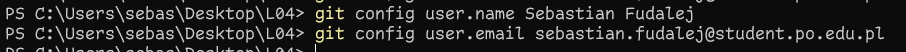
\includegraphics[width=0.8\textwidth]{image/git/1.png}
	\caption{Konfiguracja GIT}
\end{figure}

\begin{figure}[h]
	\centering
	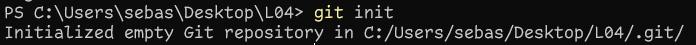
\includegraphics[width=0.8\textwidth]{image/git/2.png}
	\caption{Stworzenie lokalnego repozytorium}
\end{figure}

\begin{figure}[h]
	\centering
	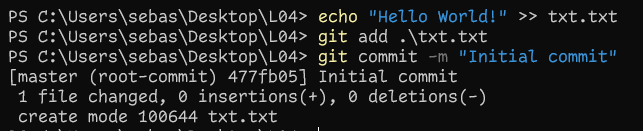
\includegraphics[width=0.8\textwidth]{image/git/3.png}
	\caption{Dodanie do repozytorium dowolnych plików}
\end{figure}

\begin{figure}[h]
	\centering
	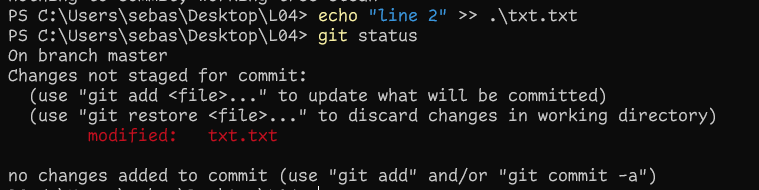
\includegraphics[width=0.8\textwidth]{image/git/4.png}
	\caption{Wprowadzenie zmian w plikach}
\end{figure}

\begin{figure}[h]
	\centering
	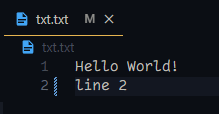
\includegraphics[width=0.8\textwidth]{image/git/5.png}
	\caption{Zmiany w pliku w edytorze tekstowym}
\end{figure}

\begin{figure}[h]
	\centering
	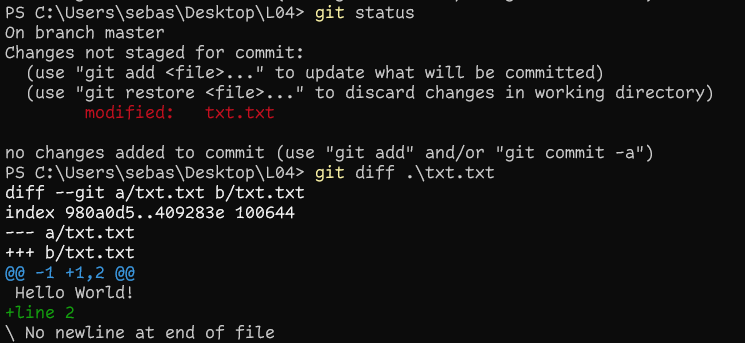
\includegraphics[width=0.8\textwidth]{image/git/6.png}
	\caption{Diff - porównanie zmian w plikach}
\end{figure}

\begin{figure}[h]
	\centering
	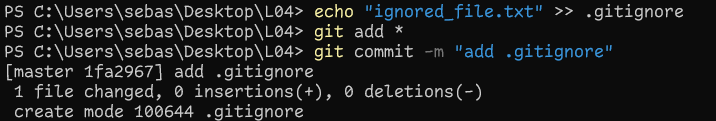
\includegraphics[width=0.8\textwidth]{image/git/7.png}
	\caption{Dodanie pliku .gitignore}
\end{figure}

\begin{figure}[h]
	\centering
	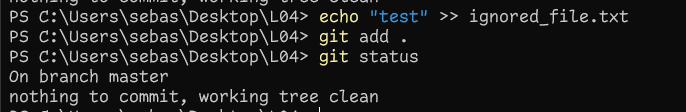
\includegraphics[width=0.8\textwidth]{image/git/8.png}
	\caption{Stworzenie ignorowanego pliku}
\end{figure}

\begin{figure}[h]
	\centering
	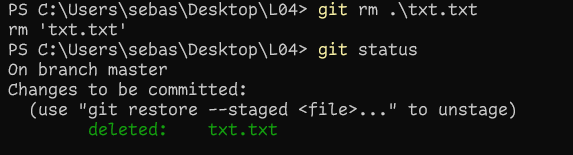
\includegraphics[width=0.8\textwidth]{image/git/9.png}
	\caption{Usunięcie pliku}
\end{figure}

\begin{figure}[h]
	\centering
	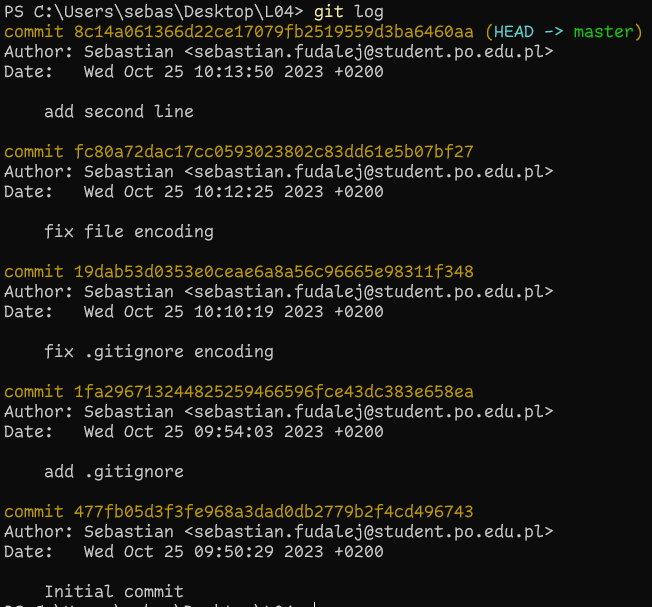
\includegraphics[width=0.8\textwidth]{image/git/10.png}
	\caption{Historia rewizji}
\end{figure}

\begin{figure}[h]
	\centering
	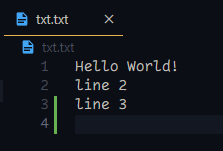
\includegraphics[width=1\textwidth]{image/git/11.png}
	\caption{Modyfikacja pliku}
\end{figure}

\begin{figure}[h]
	\centering
	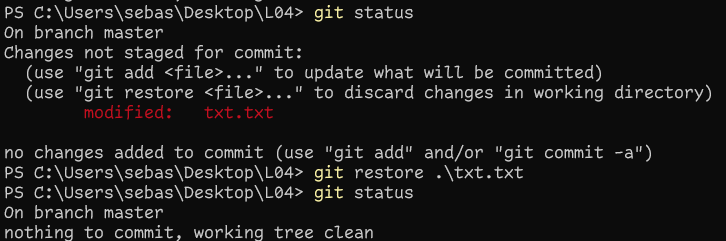
\includegraphics[width=1\textwidth]{image/git/12.png}
	\caption{Cofnięcie zmian w pliku}
\end{figure}

\begin{figure}[h]
	\centering
	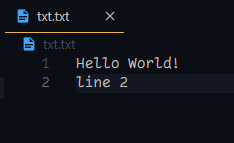
\includegraphics[width=1\textwidth]{image/git/13.png}
	\caption{Plik po przywróceniu zmian}
\end{figure}

\begin{figure}[h]
	\centering
	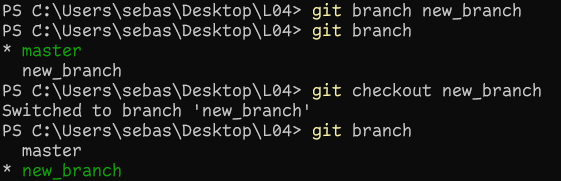
\includegraphics[width=1\textwidth]{image/git/14.png}
	\caption{Stworzenie nowego brancha}
\end{figure}

\begin{figure}[h]
	\centering
	
\includegraphics[width=1\textwidth]{image/git/15.png}
	\caption{Stworzenie nowego pliku}
\end{figure}

\begin{figure}[h]
	\centering
	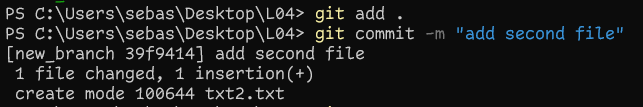
\includegraphics[width=1\textwidth]{image/git/16.png}
	\caption{Dodanie pliku do nowego brancha}
\end{figure}

\begin{figure}[h]
	\centering
	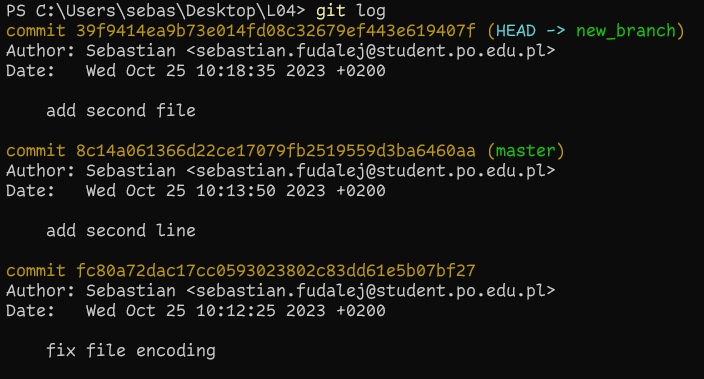
\includegraphics[width=1\textwidth]{image/git/17.png}
	\caption{Git log po commicie na nowym branchu}
\end{figure}

\begin{figure}[h]
	\centering
	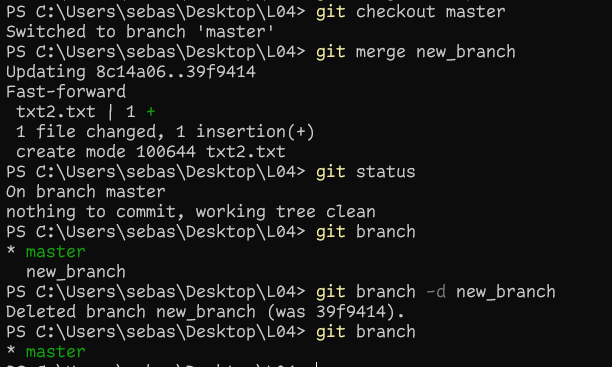
\includegraphics[width=1\textwidth]{image/git/18.png}
	\caption{Przejście na mastera i zmergowanie brancha}
\end{figure}

\begin{figure}[h]
	\centering
	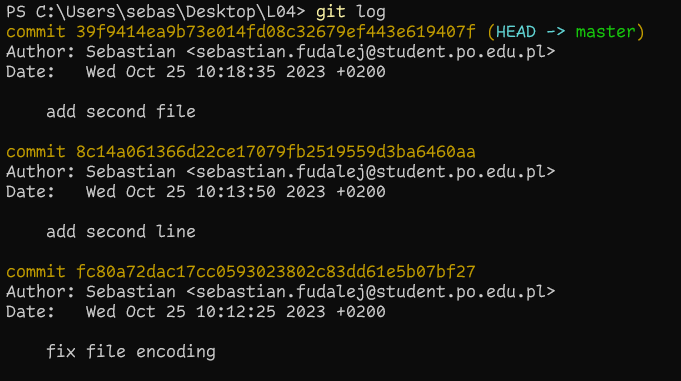
\includegraphics[width=1\textwidth]{image/git/19.png}
	\caption{Git log po zmergowaniu brancha}
\end{figure}

\begin{figure}[h]
	\centering
	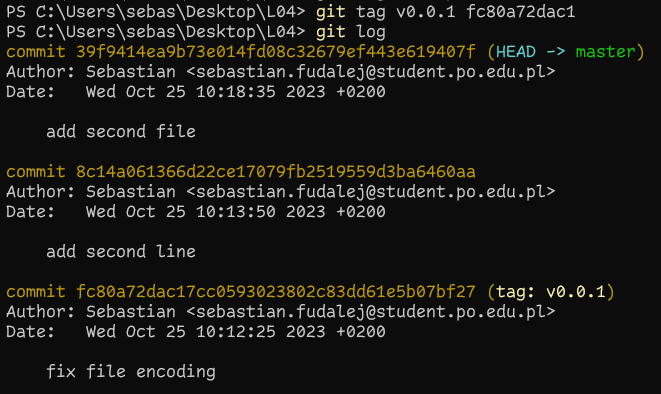
\includegraphics[width=1\textwidth]{image/git/20.png}
	\caption{Tagowanie danego commita}
\end{figure}

\begin{figure}[h]
	\centering
	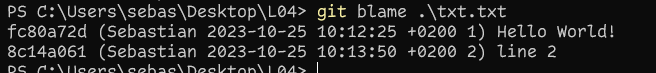
\includegraphics[width=1\textwidth]{image/git/21.png}
	\caption{Git blame}
\end{figure}

\begin{figure}
	\centering
	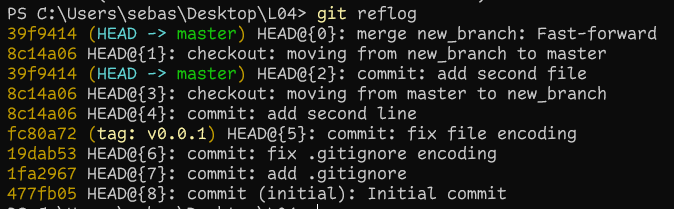
\includegraphics[width=1\textwidth]{image/git/22.png}
	\caption{Git reflog}
\end{figure}

\begin{figure}
	\centering
	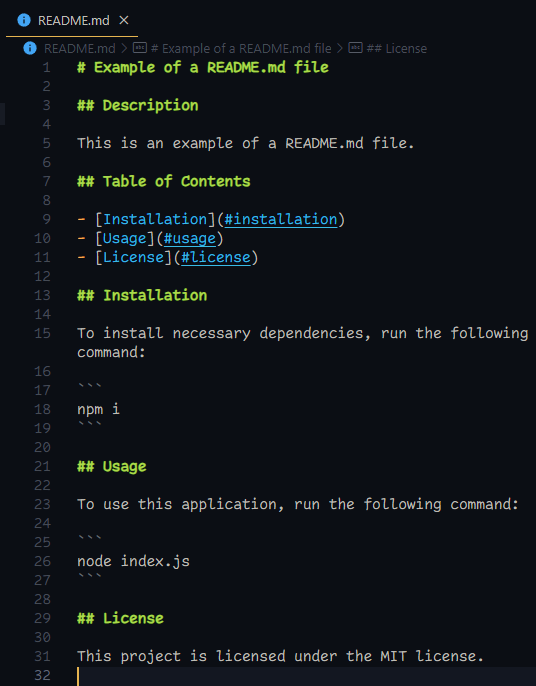
\includegraphics[width=1\textwidth]{image/git/23.png}
	\caption{Dodanie README.md}
\end{figure}

\begin{figure}
	\centering
	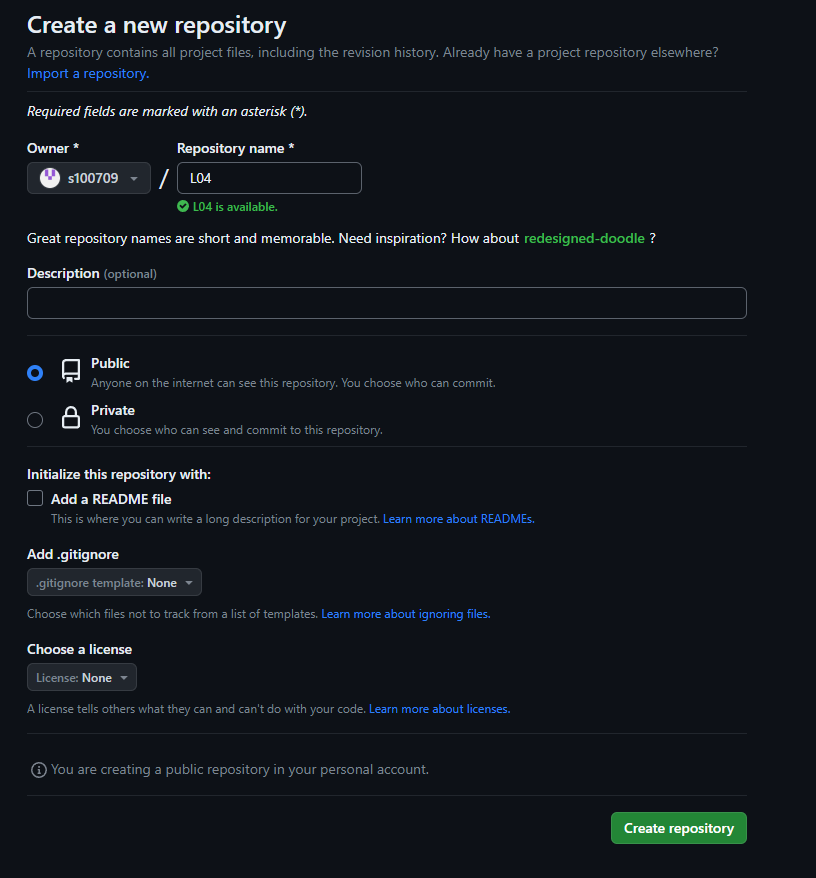
\includegraphics[width=1\textwidth]{image/git/24.png}
	\caption{Stworzenie repozytorium na GitHubie}
\end{figure}

\begin{figure}
	\centering
	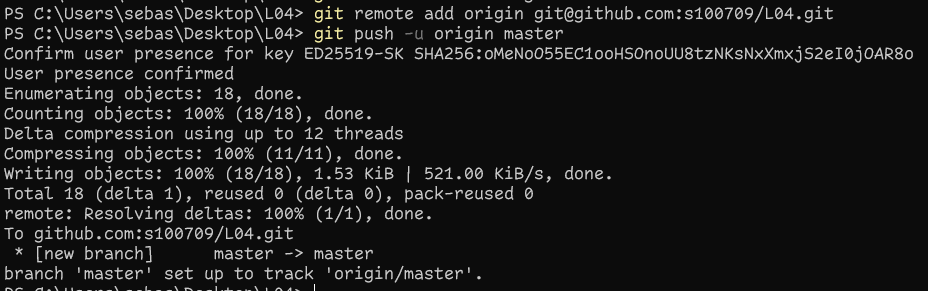
\includegraphics[width=1\textwidth]{image/git/25.png}
	\caption{Dodanie remote do lokalnego repozytorium}
\end{figure}

\begin{figure}
	\centering
	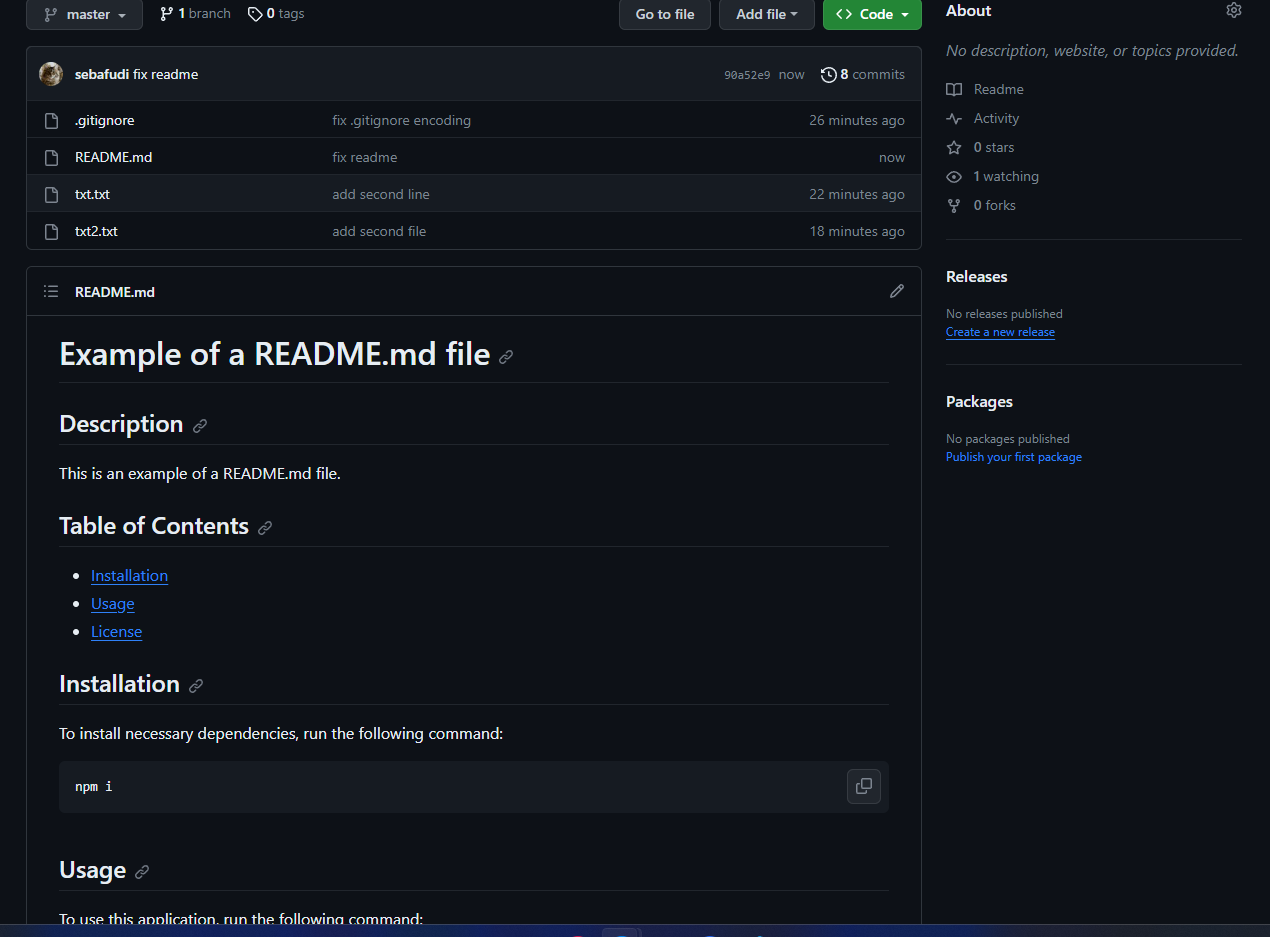
\includegraphics[width=1\textwidth]{image/git/26.png}
	\caption{Wynik na GitHubie}
\end{figure}

\end{document}